% 18 variables in here:
% h_1 = 1000.0, h_2 = 1000.0, h_3 = 1000.0, h_4 = 1000.0, h_5 = 1000.0, h_6 = 1000.0, ux_1 = 0.0, ux_2 = 0.0, ux_3 = 0.0, ux_4 = 0.0, ux_5 = 0.0, ux_6 = 0.0, uy_1 = 0.0, uy_2 = 0.0, uy_3 = 0.0, uy_4 = 0.0, uy_5 = 0.0, uy_6 = 0.0
\begin{figure}[h!]
\centering
  \subfigure[] {
    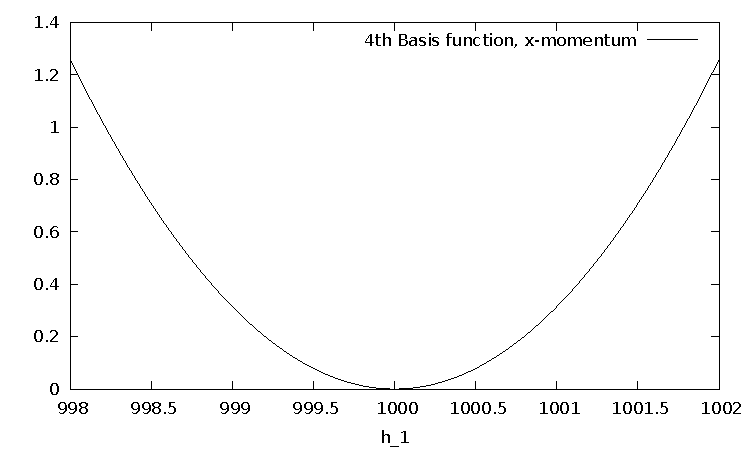
\includegraphics[scale=\zoomfactor]{{{ord2_magnitude_1000_default/y_1000.0_1000.0_1000.0_1000.0_1000.0_0.0_0.0_0.0_0.0_0.0_0.0_0.0_0.0_0.0_0.0_0.0_0.0f06}}}
  }
  \subfigure[] {
    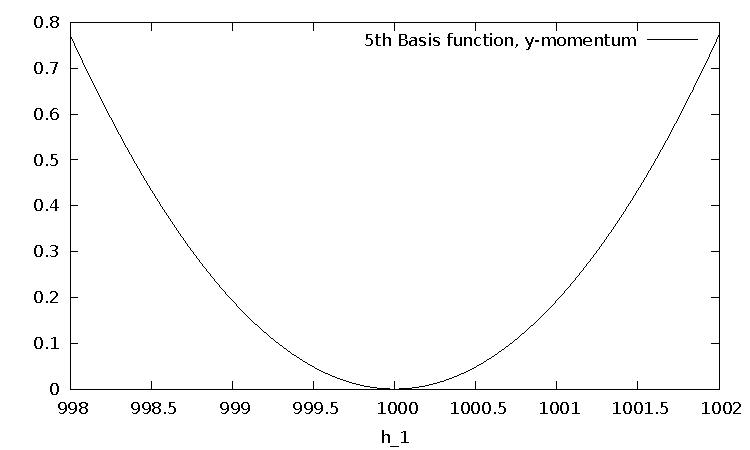
\includegraphics[scale=\zoomfactor]{{{ord2_magnitude_1000_default/y_1000.0_1000.0_1000.0_1000.0_1000.0_0.0_0.0_0.0_0.0_0.0_0.0_0.0_0.0_0.0_0.0_0.0_0.0f09}}}
  }
\caption{}
\label{fig:ord2_magnitude_1000_default}
\end{figure}

%%% Local Variables:
%%% TeX-master: "../results.tex"
%%% End:
